\section{Arquitectura general}

La Figura \ref{fig:arquitectura-open-glove}, muestra la arquitectura general de OpenGlove, donde es posible ver el trabajo previo realizado por \cite{tesis-monsalve-rodrigo}, \cite{tesis-meneses-sebastian} y \cite{tesis-cerda-rodrigo}, como también el trabajo que resulta de este proyecto y el que se realizará en un futuro.

\begin{figure}[H]
  \begin{center} 
   	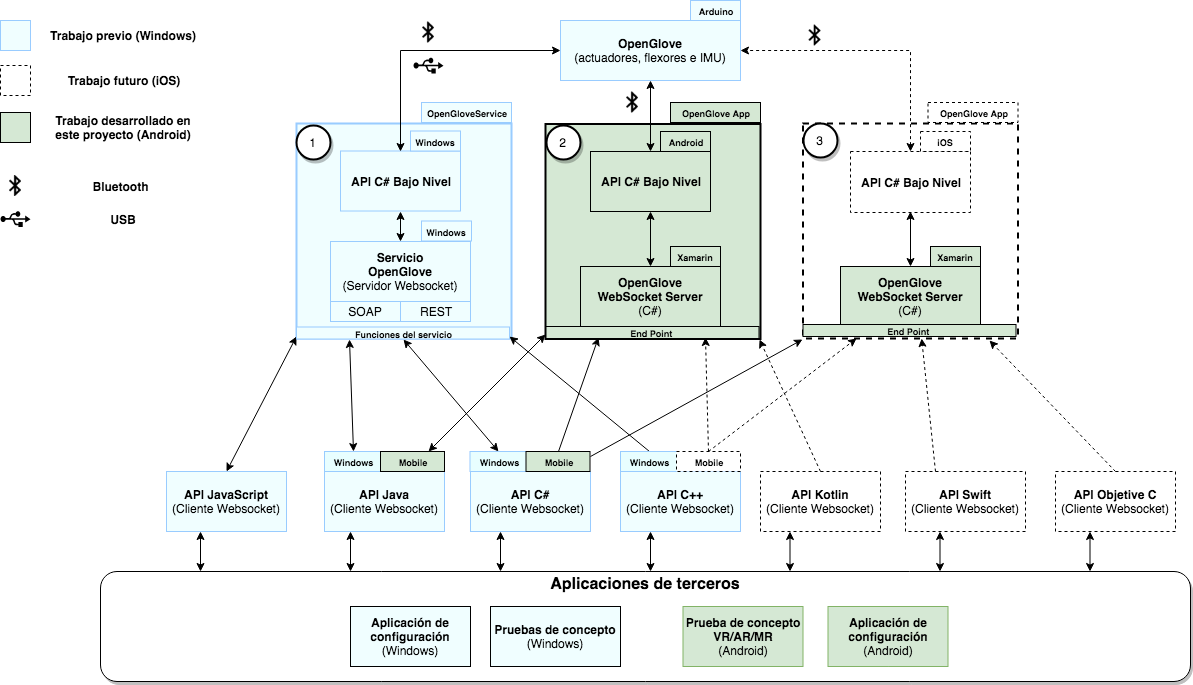
\includegraphics[width=1.0\textwidth]{images/chapter04/OpenGlove-Architecture-General.png} 
    \caption[Arquitectura de Openglove]{Arquitectura de OpenGlove \\Fuente: Elaboración propia (2018)}
    \label{fig:arquitectura-open-glove}
  \end{center}
\end{figure}

OpenGloveService  desarrollado en este proyecto, permite comunicarse con dispositivos OpenGlove a través de comunicación serial Bluetooth, accediendo a las funciones del servicio con las APIs. Éstas pueden ser utilizadas en cualquier aplicación compatible con el lenguaje de la API a utilizar. Dado que se utiliza Xamarin.Forms para desarrollar aplicaciones nativas multiplataforma, para iOS y Android, el servidor Websocket es desarrollado con C\# para que ambas plataformas compartan el código. La API de bajo nivel, debe ser específica en cada sistema operatio, por las diferencias de comunicación presentes en cada una. Por esta misma razón se desarrollan las APIs Java y C\# específicas para dispositivos móviles. La primera permite hacer uso de OpenGlove en proyectos Android y la segunda permite hacer aplicaciones para iOS y Android utilizando Xamarin. El uso de Xamarin.Forms permite reutilizar código de la Interfaz de Usuario y desarrollar de manera específica para cada plataforma utilizando C\#, haciendo referencias a las APIs específicas de cada plataforma.
